\documentclass[12pt,fleqn]{article}\usepackage{../../common}
\begin{document}
Giriş

Bu yazıda ileride hocanın tam değinmediği konuları tanıştırmaya uğraşacağız.

Vektörler

Bir vektör bir yön ve büyüklüktür, başlangıç noktası olarak genellikle orijin
kabul edilir. 1,2, ya da daha fazla boyutta bir sayı listesi ile gösterilebilir,
tek boyutta ise bu tabii ki bir skalar ile aynı şeydir [5]. 

Toplamak

İki boyutta bir örnek görelim, iki vektör $a,b$ var, toplamları

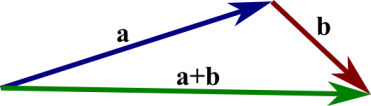
\includegraphics[width=15em]{vector_a_plus_b.png}

Toplam sanki birinci vektörü alıp diğerinin bittiği yerden başlatmak gibi,
varılan yeri gösteren yeni vektör toplam vektörüdür. Çıkartmak ise aynı yerden
başlayan iki vektörde birinin sonundan diğerine sonuna giden vektörü bulmak
gibidir. Aslında toplam üzerinden çıkartma doğrulabilir, $a-b$ düşünürken $-b$
diye yeni bir vektör yaratırız (yani vektörü tersine çeviririz) ve $a+(-b)$ ile
toplam işlemini yaparız.

Çıkartmak

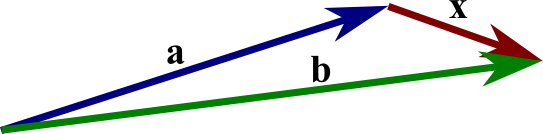
\includegraphics[width=15em]{vector_b_minus_a.png}

Kosinüsler Kanunu (Law of Cosines)

Şöyle bir üçgen olduğunu düşünelim [1],

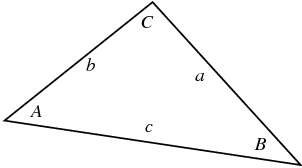
\includegraphics[width=15em]{cos1.png}

Eğer, mesela C'nin 90 derece olduğunu bilseydik, Pitagor kuralından

$$
c^2 = a^2 + b^2
$$

diyebilirdik. Ama $C < 90$ ise, farklı bir formül kullanılabilir,

$$
c^2 = a^2 + b^2 - 2 a b \cos C
$$

Eğer $C=90$ ise $\cos(90) = 0$ olduğu için Pitagor kuralını elde ettiğimizi
görürüz. 

Üstteki kurala Kosinüsler Kanunu denir, ispatı şöyle,

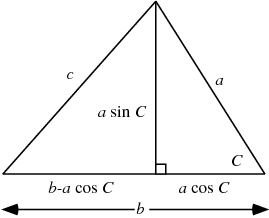
\includegraphics[width=15em]{cos2.png}

Üstteki üçgene bakarsak,

$$
c^2 = (a \sin C)^2 + (b-a\cos C)^2
$$

$$
= a^2 \sin^2 C + b^2 - 2 a b \cos C + a^2 \cos^2 C
$$

$$
c^2 = a^2 + b^2 - 2 a b \cos C
$$

Noktasal Çarpım

İki boyutta iki vektör $\vec{a},\vec{b}$ olduğunu düşünelim. Bu vektör ögelerini
$\vec{a} = [a_1, a_2]$ ve $\vec{b} = [b_1, b_2]$ diye gösterirsek, noktasal
çarpım $\vec{a} \cdot \vec{b}$ her iki vektörün tekabül eden öğelerinin
çarpımının toplamıdır, yani

$$
\vec{a} \cdot \vec{b} = a_1 b_1 + a_2 b_2
$$

Daha yüksek boyutlarda benzer işlem devam ettirilir. 

Norm

Bir vektorun uzunlugunun, buyuklugunun, ya da normu, ki $||\vec{a}||$ ile
gosterilebilir, karesi

$$
||\vec{a}||^2 = \vec{a} \cdot \vec{a} 
$$

Bu kurallara uygun çünkü

$$
(\vec{a} \cdot \vec{a})^2 = a_1 a_1 + a_2 a_2
$$

Ya da

$$
||\vec{a}|| = \sqrt{\vec{a} \cdot \vec{a}} = \sqrt{a_1 a_1 + a_2 a_2}
$$

Aslında büyüklük formülü Pitagor üçgen formülünden hareketle de anlaşılır çünkü
herhangi bir vektör düşünürsek, $a_1,a_2$ ya da $x$ ekseninde $a_1$ $y$
ekseninde $a_2$ olan bir nokta düşünürsek bu noktaya olan orijinden olan uzaklık
(vektör) Pitagor formülü ile hesaplanabilirdi, $\sqrt{a_1^2 + a_2^2}$.

Noktasal çarpım şu şekilde de hesaplanabilir,

$$
\vec{a} \cdot \vec{b} = ||\vec{a}|| ||\vec{b}|| \cos\theta
$$

İspat

Alttaki şekle bakarsak,

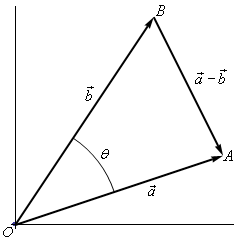
\includegraphics[width=15em]{abcos.png}

Bu üçgenin kenarları arasında Kosinüsler Kanunu uygularsak,

$$
||\vec{a}-\vec{b}||^2 =
||\vec{a}||^2 + ||\vec{b}||^2 -
2 ||\vec{a}|| ||\vec{b}|| \cos\theta
\mlabel{1}
$$

Norm açılımından hareketle

$$
||\vec{a}-\vec{b}||^2 = (\vec{a}-\vec{b}) \cdot (\vec{a}-\vec{b}) 
$$

Noktasal çarpımı parantezler üzerinden açarsak,

$$
= \vec{a}\cdot\vec{a} - \vec{a}\cdot\vec{b} - \vec{b}\cdot\vec{a} + \vec{b}\cdot\vec{b}
$$

$$
= ||\vec{a}||^2 - 2\vec{a}\cdot\vec{b} + ||\vec{b}||^2
$$

(1) formülünde sol tarafı üstteki formülle açarsak,

$$
||\vec{a}||^2 - 2\vec{a}\cdot\vec{b} + ||\vec{b}||^2 =
||\vec{a}||^2 + ||\vec{b}||^2 - 2 ||\vec{a}|| ||\vec{b}|| \cos\theta
$$

$$
- 2\vec{a}\cdot\vec{b} = - 2 ||\vec{a}|| ||\vec{b}|| \cos\theta
$$

$$
\vec{a}\cdot\vec{b} = ||\vec{a}|| ||\vec{b}|| \cos\theta
$$

Üstteki eşitlik veri analizinde kullanışlı bulunmuştur, mesela kimisi
müşterileri $D$ boyutunda vektörler olarak temsil edebilir, 1. öğe yaş, 2. öğe
boy, vs. gibi bilgiler olabilir ve iki vektörün birbirine ne kadar ``yakın''
olduğu iki vektörün arasındaki açısal uzaklık üzerinden ölçülebilir,

$$
\cos\theta = \frac{\vec{a}\vec{b}}{||\vec{a}|| ||\vec{b}||}
$$

Eğer vektörler baştan normalize edilmiş ise bölme işlemine de gerek kalmaz, tek
bir noktasal çarpım ile kabaca bir benzerlik ölçütü elde edilmiş olur.

Bir diğer kullanım alanı fizikte ``yapılan iş'' hesabı. İş, uygulanan kuvvet
çarpı mesafeden elde edilir fakat mesela bir kuvvet alanı $\vec{F}$ her yerde
farklı olabilir ayrıca bu alanda belli bir $\vec{d}$ yolunda hareket eden bir
parçacığı düşünürsek, parçacık bazen kuvvete karşı bazen onunla beraber hareket
ediyor olabilir, bunun ne oranda olduğunun hesabı $\vec{F}$'yi $\vec{d}$ üzerine
skalar olarak yansıtmakla hesaplanır [3], $W = \vec{F} \cdot \vec{d}$.

Diklik

İki vektörün birbirine dik olup olmadığı (orthogonality) testi de noktasal
çarpım ile yapılır. $\cos(90) = 0$ olduğuna göre $\vec{a}\cdot\vec{b}$ çarpımı
sıfır ise iki vektör dik demektir. 

Yansıtma (Projection)

Vektör $\vec{a}$'nin $\vec{b}$ yönündeki büyüklüğü, yansıması nedir sorusunun
cevabı da noktasal çarpım ile bulunabilir, 

$$
\vec{a}\cdot\vec{b} = ||\vec{a}||||\vec{b}||\cos\theta
$$

formülünü biraz manipüle edersek cevabı alabiliriz, 

$$
\frac{\vec{a}\cdot\vec{b}}{||\vec{b}||} = ||\vec{a}|| \cos \theta
$$

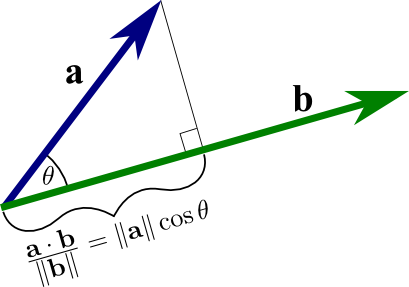
\includegraphics[width=15em]{dot_product_projection.png}

Eşitliğin sağ tarafı $||\vec{a}|| \cos \theta$ aradığımız büyüklük, onu elde
etmek için $\frac{\vec{a}\cdot\vec{b}}{||\vec{b}||}$ noktasal çarpımını
kullanabileceğimizi görüyoruz [4].

Eğer büyüklüksel, skala yansımasını bulabiliyorsak, bir vektörün diğeri
yönündeki tamamen yansımasını da bulabilirdik, $\vec{b}$ yönünü
$\frac{\vec{b}}{||\vec{b}||}$ birim vektörü ile gösteriyoruz, o yöndeki
$\vec{a}$ büyüklüğünü biraz önce bulduk, $\frac{\vec{a}\cdot\vec{b}}{||\vec{b}||}$.

Yönü büyüklük ile çarpınca istenilen vektör elde edilmiş olur [3], $\vec{a}$'nin
$\vec{b}$ yönündeki yansıması $\proj_{\vec{b}} \vec{a}$

$$
\proj_{\vec{b}} \vec{a} = \frac{\vec{a}\cdot\vec{b}}{||\vec{b}||} \frac{\vec{b}}{||\vec{b}||}
$$

$$
= \frac{\vec{a}\cdot\vec{b}}{||\vec{b}||^2} \vec{b}
$$

Baz Değişimi

Aksi belirtilmediği sürece verili herhangi bir matrisin standart $i,j,k,..$ baza
sahip olduğu kabul edilir, bu sayede mesela $[\begin{array}{cc}1&2\end{array}]$
vektörünü $i$'dan 1 tane $j$'den iki tane şeklinde gösterebiliriz [6].

Her temel baz tek bir eksen icin 1 digeri icin 0 degerindedir,

$$
i = \left[\begin{array}{c}1 \\ 0 \end{array}\right], \quad
j = \left[\begin{array}{c}0 \\ 1 \end{array}\right]
$$

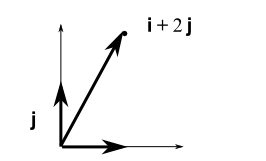
\includegraphics[width=15em]{ijbasis.png}

2 boyutta herhangi bir matrisin aslında bu ``standart baz üzerinden''
tanımlanmış olduğu kabul edilir,

$$
Bx = 
\left[\begin{array}{ccc}
1 & 0 \\ 0 & 1
\end{array}\right]
\left[\begin{array}{c}
x_1 \\ x_2
\end{array}\right] =
x_1 \left[\begin{array}{c}
1 \\ 0
\end{array}\right] +
x_2 \left[\begin{array}{c}
0 \\ 1
\end{array}\right]
$$

Bu bakış açısı faydalı çünkü böylece herhangi bir transformasyona baz değişimi
olarak bakılabilir, tek gereken yeni $i$, ve yeni $j$'nin (daha üst boyutlarda
$k$, vs) nereye işaret ettiğini bilmek. Mesela kaykılma (shear)
transformasyonunu alırsak, tüm dünyayı 45 derece sağa kaydırmak istiyoruz, bunun
için yeni $i,j$

$$
i = \left[\begin{array}{c}1 \\ 0 \end{array}\right], \quad
j = \left[\begin{array}{c}1 \\ 1 \end{array}\right]
$$

Bu bazla soldan çarparsak, mesela bir $[\begin{array}{cc}1&2\end{array}]^T$ vektörü,

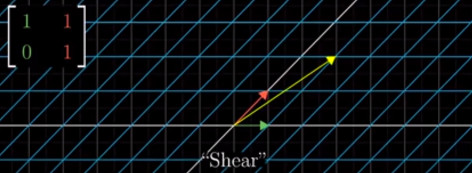
\includegraphics[width=20em]{shear.jpg}

haline gelir.

Baz Değişimi Bakışı Açısı ve Yansıtma

Yansıtmayı baz değişimi (change of basis) olarak görürsek ilginç bir görüşe daha
kavuşuyoruz. Biliyoruz ki $x$ vektörünü transforme edip yeni bir $B$ bazına
taşımak için $x$'i soldan çarpmak yeterli, mesela

$$
Bx = 
\left[\begin{array}{ccc}
a & b \\ c & d
\end{array}\right]
\left[\begin{array}{c}
x_1 \\ x_2
\end{array}\right] =
x_1 \left[\begin{array}{c}
a \\ c
\end{array}\right] +
x_2 \left[\begin{array}{c}
b \\ d
\end{array}\right]
$$

Her ayri baz $B$ kolonlari icinde, her kolon 2 boyutlu, yani 2 boyuttan 2 boyuta
baz degisimi yapmis olduk. Fakat boyut degisimi de olabilirdi, mesela 

$$
Bx = 
\left[\begin{array}{ccc}
a & b 
\end{array}\right]
\left[\begin{array}{c}
x_1 \\ x_2
\end{array}\right] =
x_1 \left[\begin{array}{c}
a 
\end{array}\right] +
x_2 \left[\begin{array}{c}
b 
\end{array}\right]
$$

Son çarpımlar 1x1 boyutlu ``matrisler'' içeriyor, yani bunlar skalar, ki son
toplamdan elde edilen sayı da skalar olacaktır, $x_1 a + x_2 b$. İşte noktasal
çarpım, skalar yansıtmaya bakmanın bir diğer yolu bu, bir vektör $v_1$'in bazını
değiştirip $v_2$ haline getirmek ilk vektörü ikincisi üzerinde yansıtmak
anlamına gelmez mi? 

Kaynaklar

[1] \url{https://mathworld.wolfram.com/LawofCosines.html}

[2] \url{https://tutorial.math.lamar.edu/classes/calcii/dotproduct.aspx}

[3] \url{http://sites.science.oregonstate.edu/math/home/programs/undergrad/CalculusQuestStudyGuides/vcalc/dotprod/dotprod.html}

[4] {\em Math Insight},
    \url{https://mathinsight.org/dot_product}

[5] {\em Math Insight},
    \url{https://mathinsight.org/vector_introduction}

[6] 3Blue1Brown, \url{https://www.youtube.com/watch?v=k7RM-ot2NWY}

\end{document}





